
\addcontentsline{toc}{section}{Introduction}
\section*{Introduction}

\section{About}
Izicap est un pionnier dans l'utilisation des données de cartes de paiement et les transforme en une connaissance client et des informations commerciales puissantes pour les commerçants, leur permettant de gérer leurs propres programmes de fidélité et campagnes de marketing numérique. 
Ces services marketing, fournis par les acquéreurs utilisant les solutions SaaS d'Izicap, redonnent rapidement de la croissance aux entreprises marchandes en renforçant les dépenses et la fidélité de leurs clients (les titulaires de carte). 
La solution innovante de CRM et de fidélité liée aux cartes d'Izicap donne aux acquéreurs un avantage concurrentiel en monétisant leurs données de transactions de paiement, en générant de nouvelles sources de revenus et en améliorant leurs capacités de rétention.
Après s'être solidement implanté en France grâce à des partenariats avec le Groupe BPCE et le Crédit Agricole, Izicap s'est associé à Nexi, le premier acquéreur et Fintech en Italie et a rejoint le programme StartPath de Mastercard dans le but d'étendre considérablement sa portée mondiale. 
Izicap s'associe aux principaux fournisseurs de solutions de paiement tels qu'Ingenico, Verifone, Poynt et PAX, et rend sa solution CRM et Fidélité liée à la carte disponible sur les terminaux de paiement les plus populaires et les plus innovantes.

\section{Organigramme}
\begin{figure}[H]
\centering
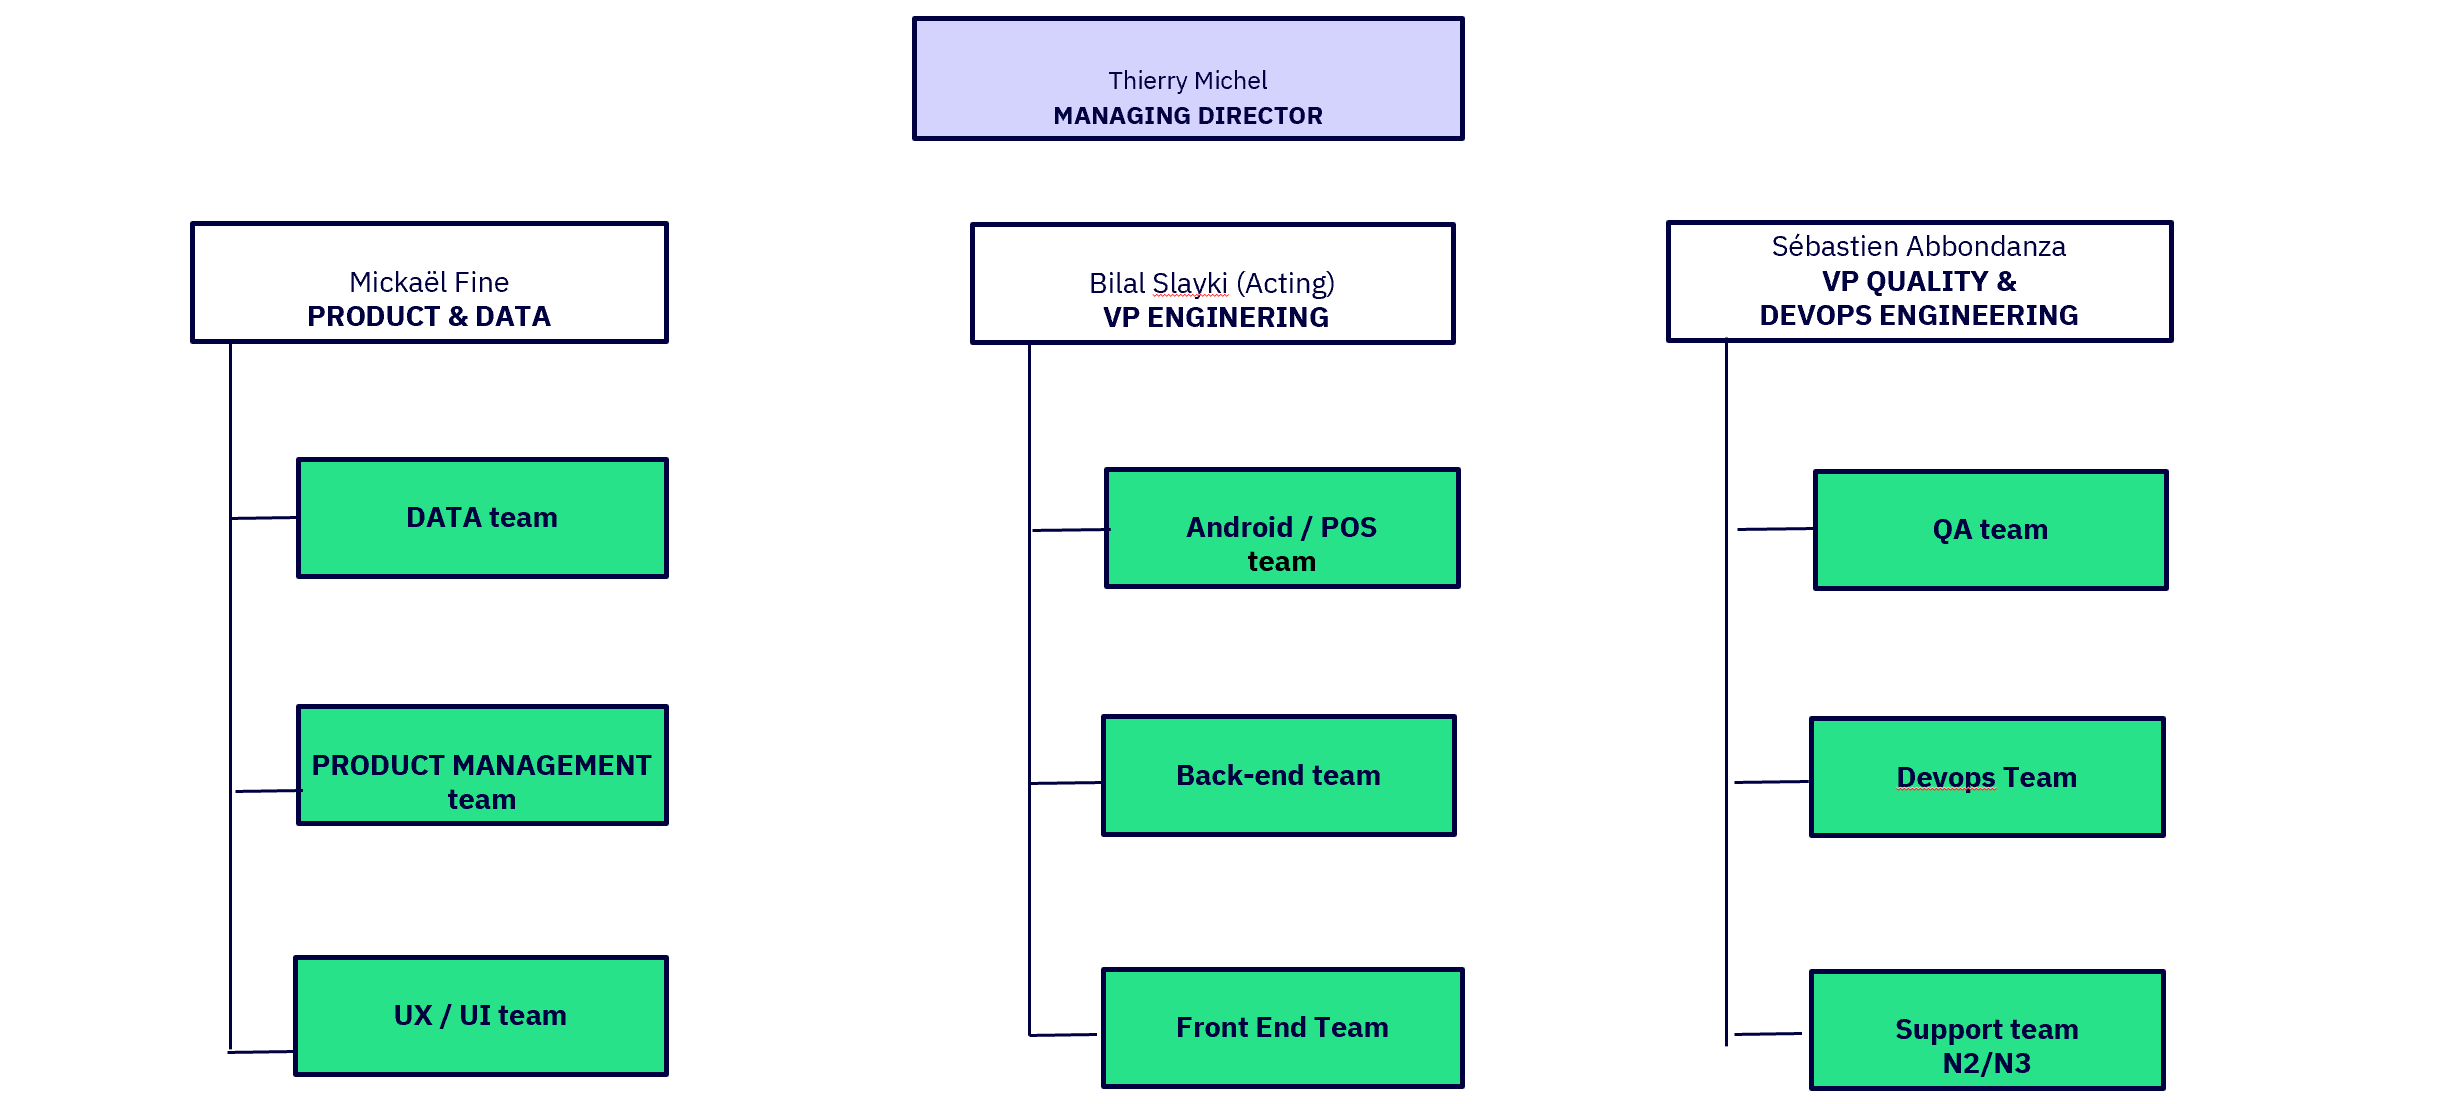
\includegraphics[width=\linewidth]{images/orga.png}
\caption{Organigramme de Izicap}\label{fig:organigmramme}
\end{figure}

\addcontentsline{toc}{section}{Conclusion}
\section*{Conclusion}
